\setchapterimage[6.5cm]{seaside}
\setchapterpreamble[u]{\margintoc}
\chapter{Figures and Tables\footnotemark[0]}

\footnotetext{The credits for the image above the chapter title go to:
	Bushra Feroz --- Own work, CC~BY-SA~4.0, 
	\url{https://commons.wikimedia.org/w/index.php?curid=68724647}}

\section{Normal figures and tables}

Figures and tables can be inserted just like in any standard 
\LaTeX\xspace document. The \Package{graphicx} package is already loaded 
and configured in such a way that the figure width is equal to the 
textwidth and the height is adjusted in order to maintaini the original 
aspect ratio. As you may have imagined, the captions will be 
positioned\ldots well, in the margins. This is achieved with the help of 
the \Package{floatrow} package.

Here is a picture of Mona Lisa (\reffig{normalmonalisa}), as an example. 
The captions are formatted as the margin- and the side-notes; If you 
want to change something about captions you can use the command 
\Command{captsetup} from the \Package{caption} package. Remember that if 
you want to reference a figure, the label must come \emph{after} the 
caption!

\begin{figure}[h]
	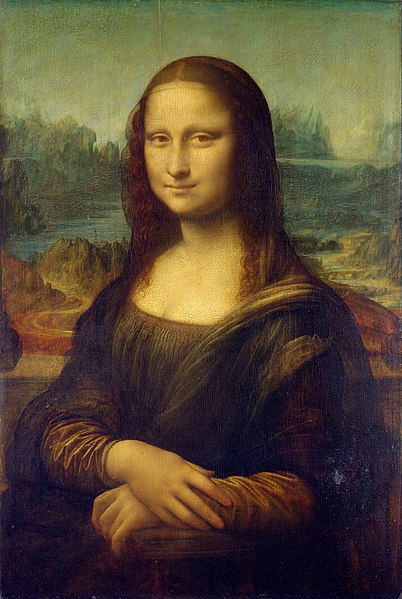
\includegraphics[width=0.45\textwidth]{monalisa}
	\caption[Mona Lisa, again]{It's Mona Lisa again. \blindtext}
	\labfig{normalmonalisa}
\end{figure}

The position of the caption, as opposed to its format, is handled by the 
\Package{floatrow} package. Achieving this result has been quite hard, 
but now I am pretty satisfied.

\begin{kaobox}[frametitle=To Do]
The only problem is that the captions will always be aligned to the 
bottom of the figure/table. I tried to follow the \Package{floatrow} 
manual, but even specifying the \enquote{\Option{top}} option, I cannot 
make it work. If you know how to fix this, please let me know.
\end{kaobox}

Tables can be inserted as easily as figures, as exemplified by the 
following code:

\begin{lstlisting}
\begin{table}
\begin{tabular}{ c c c c }
	\toprule
	col1 & col2 & col3 & col 4 \\
	\midrule
	\multirow{3}{4em}{Multiple row} & cell2 & cell3 & cell4\\ &
	cell5 & cell6 & cell7 \\ &
	cell8 & cell9 & cell10 \\
	\multirow{3}{4em}{Multiple row} & cell2 & cell3 & cell4 \\ &
	cell5 & cell6 & cell7 \\ &
	cell8 & cell9 & cell10 \\
	\bottomrule
\end{tabular}
\end{table}
\end{lstlisting}

which results in the useless \vreftab{useless}.

\begin{table}[b]
\caption[A useless table]{A useless table.}
\begin{tabular}{ c c c c }
	\toprule
	col1 & col2 & col3 & col 4 \\
	\midrule
	\multirow{3}{4em}{Multiple row} & cell2 & cell3 & cell4\\ &
	cell5 & cell6 & cell7 \\ &
	cell8 & cell9 & cell10 \\
	\multirow{3}{4em}{Multiple row} & cell2 & cell3 & cell4 \\ &
	cell5 & cell6 & cell7 \\ &
	cell8 & cell9 & cell10 \\
	\bottomrule
\end{tabular}
\labtab{useless}
\end{table}

I don't have much else to say, so I will just insert some blind text. 
\blindtext

\section{Margin figures and tables}

Marginfigures can be inserted with the environment \verb|marginfigure|. 
In this case, the whole picture is confined to the margin and the 
caption is below it. \reffig{marginmonalisa} is obtained with something 
like this:

\begin{lstlisting}
\begin{marginfigure}
	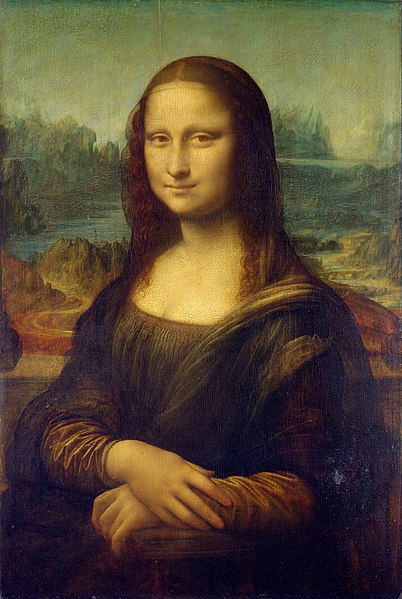
\includegraphics{monalisa}
	\caption[The Mona Lisa]{The Mona Lisa.}
	\labfig{marginmonalisa}
\end{marginfigure}
\end{lstlisting}

There is also the \verb|margintable| environment, of which 
\reftab{anotheruseless} is an example.

\begin{margintable}
\raggedright
\begin{tabular}{ c c c c }
	\hline
	col1 & col2 & col3 \\
	\hline
	\multirow{3}{4em}{Multiple row} & cell2 & cell3 \\ & cell5 & cell6 
	\\ & cell8 & cell9 \\ \hline
\end{tabular}
\caption[Another useless table]{Another useless table.}
\labtab{anotheruseless}
\end{margintable}

Marginfigures and tables can be positioned with an optional offset 
command, like so:

\begin{lstlisting}
\begin{marginfigure}[offset]
	\includegraphics{images/seaside}
\end{marginfigure}
\end{lstlisting}

Offset ca be either a measure or a multiple of \verb|\baselineskip|, 
much like with \verb|\sidenote|, \verb|\marginnote| and 
\verb|\margintoc|.\todo{improve this part} If you are wondering how I 
inserted this orange bubble, have a look at the \verb|todo| package.

\section{Wide figures and tables}

With the environments \verb|figure*| and \verb|table*| you can insert 
figures which span the whole page width. The caption will be positioned 
below.

\begin{figure*}[h!]
	\includegraphics{seaside}
	\vspace*{-1.3cm}
	\caption[A wide seaside]{A wide seaside, and a wide caption.
		Credits: By Bushra Feroz - Own work, CC BY-SA 4.0, 
		https://commons.wikimedia.org/w/index.php?curid=68724647.
		\blindtext}
\end{figure*}

\section{TikZ}

It is relatively easy to insert a figure before the chapter title with 
the help of the \verb|\setchapterpreamble| command. The details are left 
to the reader.\sidenote{Check the source code for a hint.}

In this chapter I also have used a different chapter title style. This 
is just to demonstrate how easy it is to alter the default if you don't 
like it and if you are willing to write some commands on your own. For 
instance, you could try the following code:

\begin{lstlisting}
\renewcommand*{\chapterformat}
{
  \enskip\mbox{\scalebox{3.5}{\framebox{\thechapter\autodot}}}
}
\renewcommand\chapterlinesformat[3]
{
  \parbox[b]{\textwidth+\marginparsep+\marginparwidth}{
	\parbox[b]{\textwidth}{#3}%
	\parbox[b]{\marginparsep}{\hfill}%
	\parbox[b]{\marginparwidth}{#2}%
  }
  %\hrule
}
\end{lstlisting}
